\documentclass[conference]{IEEEtran}

\usepackage{url}
\usepackage{graphicx}
\usepackage{algorithm}
% \usepackage{algorithmic}
\usepackage{algpseudocode}
\usepackage{amsmath}
\usepackage{amssymb}
\usepackage{amsthm}

\begin{document}

\title{Bitcoin Boomerang \\ {\LARGE Incentivized Anonymity for Transaction Broadcasting}}

\author{\IEEEauthorblockN{Christopher A. Wood}
\IEEEauthorblockA{Department of Computer Science\\
University of California Irvine\\
Email: woodc1@uci.edu}
\and
\IEEEauthorblockN{Chris H. Vu}
\IEEEauthorblockA{Department of Computer Science\\
University of California Irvine\\
Email: ChrisHVu@gmail.com}}

% make the title area
\maketitle

\begin{abstract}
TODO
\end{abstract}

\IEEEpeerreviewmaketitle

\section{Introduction}
%TODO: general overview of cryptocurrency, bitcoin (why it's unique), and a summary of problems it suffers from

Electronic commerce would benefit greatly from the existence of a completely secure, private, and anonymous form of digital currency that does not rely on trusted third parties or external financial institutions to manage transactions. Motivated by this ideal type of currency, there have been many research efforts focused on generating suitable cryptography-based digital payment systems, or cryptocurrencies, such as DigiCash \cite{digicash}, E-Cash \cite{ecash}, HashCash \cite{hashcash}, Namecoin \cite{namecoin}, Peercoin \cite{peercoin}, Litecoin \cite{litecoin}, Ripple \cite{ripple}, and perhaps the most popular variant, Bitcoin \cite{bitcoin}. Each of these schemes offer different tradeoffs of security, privacy, and anonymity, and as such have varying popularity among users. However, it is the distribtued, decentralized nature of Bitcoin that has led to its widespread popularity among the general public and research communities \cite{news articles}. 

Bitcoin is distinguished from other cryptocurrencies by the fact that it does not rely on trusted third parties. Specifically, the global and publicly accessible ledger that stores records of all financial transactions, thereby serving as a verifiable history of all Bitcoin funds in circulation, is maintained by a widely distributed, peer-to-peer network of (untrusted) users. Transactions are linked to specific identities, or pseudonyms, via digital signatures used to ensure the validity of each transaction. In this context, it is often convenient to associate specific pseudonomous addresses with a single public and private key pair owned by a particular user. Unfortunately, these pseudonoyms are very weak masks for the underlying user's identity - user privacy and anonymity are still at risk even with the use of such pseudonomous identities. This is true even if a user has multiple pseudononyms and uses them with caution to deter attackers looking for such links. Consequently, user deanonymization is a major problem for Bitcoin users, and there have been several academic efforts to further the cause for Bitcoin user privacy and anonymity, including studies by Reid and Harrigan \cite{ReidHarrigan13} and Androulaki et al. \cite{Androulaki12-privacy}, and we can expect to see similar work publishing in the coming years. Elias \cite{8} also discussed some legal, and moral, aspects of the anonymity, or lack thereof, in Bitcoin. We do not focus on such legality issues here, and merely operate under the assumption that spender anonymity is an ideal property that any currency system should have.

Currently, techniques to address such anonymity issues with Bitcoin are rather limited and include the use of Chaumian's entirely independent e-cash system \cite{chaumain}, which relies on trusted third parties, and Zerocoin \cite{zerocoin}, which achieves privacy and anonymity properties based on strong cryptographic assumptions at the protocol-level by working \emph{on top of} Bitcoin, among others. The former is not ideal for several reasons; the most significant of which is that it directly conflicts with the decentralized nature of Bitcoin. The latter technique is very young, having only been published in the past year, and is just now starting to gain considerable attention \cite{pinocchio}. 

In this work we survey Bitcoin and related forms of cryptocurrency with respect to their privacy and anonymity properties. We analyze proposed solutions and offer critical insight into the open problems and difficulties in achieving perfect privacy and anonymity with minimal resource consumption (e.g., bandwidth, CPU cycles, etc.). We hope that this survey will motivate continued research on this critical problem that has the potential to change financial instutitions and forms of currency for future generations.

\todo[inline]{outline the sections here}
\section{Bitcoin Overview and Privacy Limitations}
% TODO: specific discussion of aspects of bitcoin that pertain to privacy/anonymity

TODO: intro

\subsection{Bitcoin Basics}

Bitcoin is a distributed, decentralized form of cryptocurrency. Accordingly, this enables all (digitally signed)  transactions between two parties to be conducted in a peer-to-peer fashion without the inclusion of a trusted third party, such as a bank or other financial institution. This form of decentralized exchange comes at a price, however, as there must be some way to prevent users from \emph{double spending}, or using the same funds to simultaneously pay multiple parties. Bitcoin achieves this property by relying on its users to construct a history for every transaction that takes place in the system. If a majority of the users accept the validity of a particular transaction, or a set of transactions, the global history of the system is affirmatively updated and ``confirmed'' via a cryptographic hash digest that all users agree upon. This hash digest, referred to as a hash-based proof-of-work, is what constitutes the validity of the system. By the properties of the underlying hash function, the history of the system cannot be changed without breaking the function (i.e., finding collisions) or re-doing the proof-of-work, which is computationally infeasible for small groups of nodes. Therefore, so long as a majority of the Bitcoin users are honest, the system history is deemed correct and thus all signed transactions are verified, preventing double spending by potentially malicious users participating in direct, peer-to-peer transactions. 

Unfortunately, while the above scheme is semantically correct and provides strong guarantees that all financial transactions are valid, there are inherent limitations in the amount of user privacy and anonymity that can be achieved in Bitcoin. In order to adequately define these limitations, we first describe how Bitcoin transactions are generated and how the system history is maintained. For simplicity, consider the scenario in which user $A$ wants to send $N$ BTCs (Bitcoins) to user $B$. Rather than identify users by name, Bitcoin uses \emph{addresses} that are tied to specific users to use in such transactions. Denote $\mathsf{addr}_A$ and $\mathsf{addr}_B$ as the addresses of users $A$ and user $B$ used in this transaction. It is often convenient to think of Bitcoin addresses as public keys $\mathsf{pk}_A$ and $\mathsf{sf}_B$, and as such there are corresponding private keys, which we denote as $\mathsf{sk}_A$, and $\mathsf{sk}_B$, respectively.

Structurally, a transaction $T$ is a tuple comprised of the \emph{source} transactions which supplied the funds necessary to make this transaction, denoted as $\mathsf{source}$, the (public) address of the recipient, $\mathsf{addr}_B$, the amount of BTCs to send, $N$, and a digital signature of these three properties, $\mathsf{Sign}_{\mathsf{sk_A}}({\mathsf{source}, \mathsf{pk}_B, N})$. In other words, we have 
\begin{align*}
T = (\mathsf{source}, \mathsf{pk}_B, N, \sigma), 
\end{align*}
where $\sigma = \mathsf{Sign}_{\mathsf{sk_A}}({\mathsf{source}, \mathsf{pk}_B, N})$. Note that this signature is embedded in $T$ so that any other Bitcoin user may verify the validity of the content using $\mathsf{pk}_A$. Also note that $\mathsf{source}$ need not be a single transaction; user $A$ is free to use multiple transactions in order to fund their transaction to $B$. In addition to the $N$ BTC transfer from $A$ to $B$, there is often $C$ BTC amount specified in the transaction for a particular address, where $C$ denotes the amount of change that will be given to this address as a result of the transaction. It is not required that the address to which $C$ is addressed is the same as the address of $A$, though this often happens in practice. Figure \ref{fig:transaction-io} illustrates the input and output relation of our transaction from $A$ to $B$, and Figure \ref{fig:transaction-create} illustrates the steps used in constructing this transaction. Note that, in both cases, $\mathsf{source}$ is comprised of two transactions $T_1$ and $T_2$, and the resulting transaction is denoted as $T_3$.

\begin{center}
\begin{figure}
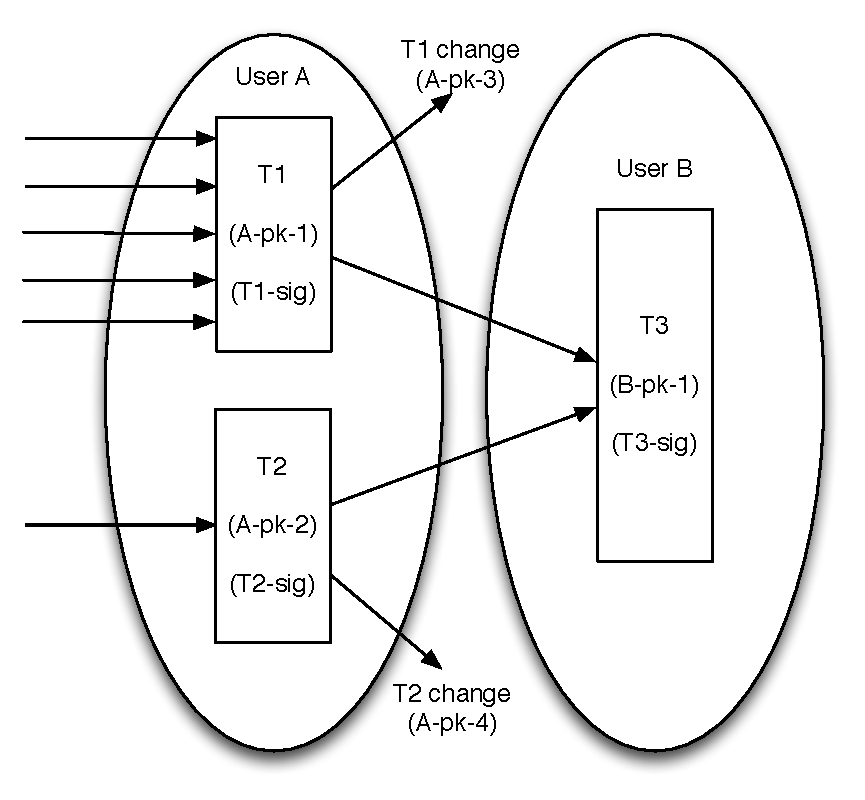
\includegraphics[scale=0.5]{./images/transaction_io.pdf}
\caption{Visual depiction of the input and output elements of a transaction from user $A$ to user $B$.}
\label{fig:transaction-io}
\end{figure}
\end{center}

\begin{center}
\begin{figure}
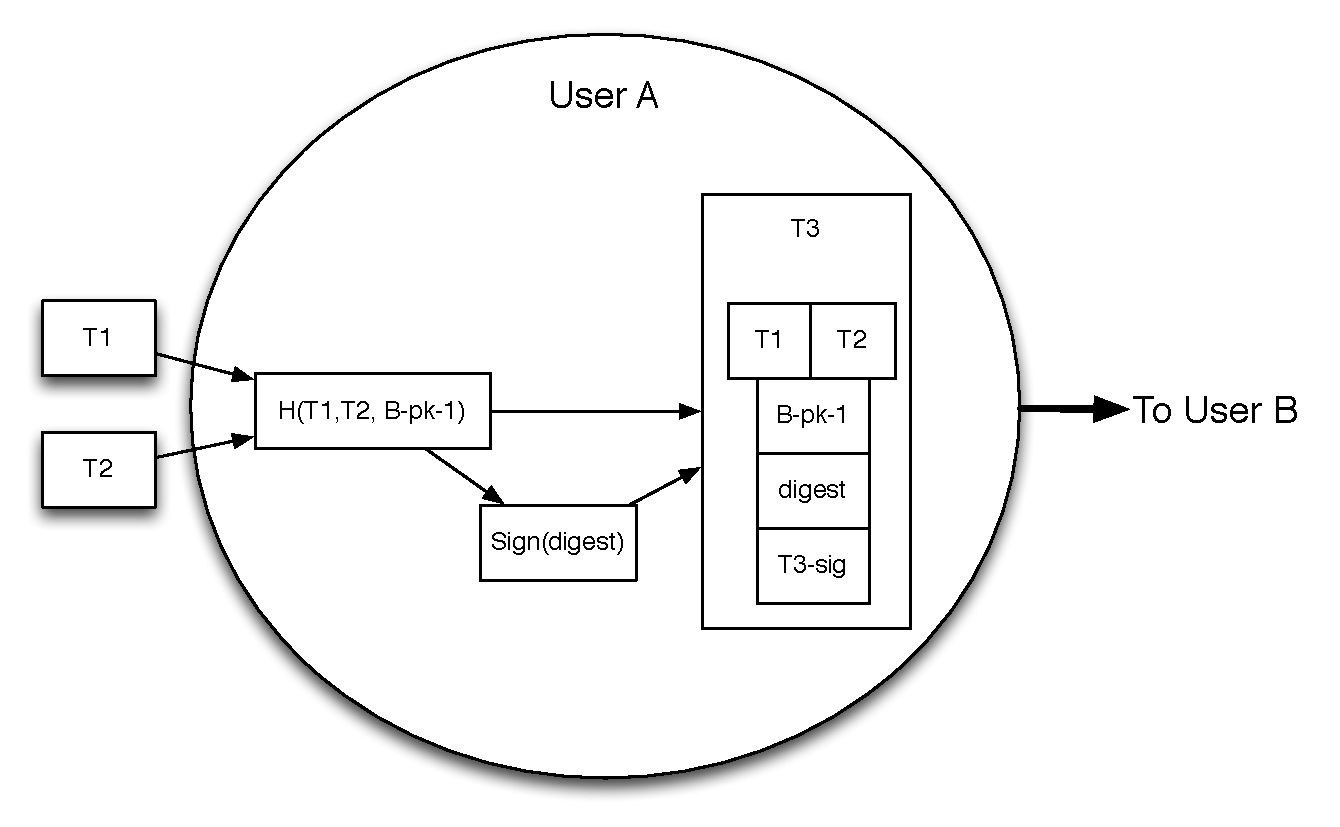
\includegraphics[scale=0.4]{./images/transaction_create.pdf}
\caption{Visual depction of the steps to create a transaction $T_3$ from user $A$ to user $B$ using two input transactions, $T_1$ and $T_2$.}
\end{figure}
\end{center}

After a transaction has been created, it is broadcasted in the network. In order to prevent double spending, nodes must confirm this transaction and append it to the chain of accepted transactions in the system's history. This procedure is based on the aforementioned proof-of-work, which works as follows. Bitcoin miners will collect unconfirmed transactions into a buffer, along with the longest chain of system-wide accepted transactions, and compute a Merkle hash of the transactions and digest of the chain. The output digest of this Merkle hash, referred to as the challenge $c$ in the proof-of-work protocol, is then used to find the proof $p$. Together, $c$ and $p$ have the property that, when concatenated and hashed using a cryptographically strong collision-resistant hash function $H$, the leading $B$ bits of the output $x = H(c || p)$ are all $0$. That is, $x = \{0,1\}^B\{0,1\}^{256-B}$. Given the collision resistant properties of $H$, finding a valid proof $p$ for the challenge $c$ is comptuationally difficult. Figure \ref{fig:block} illustrates the construction of $c$ and $p$ using a previously confirmed block chain $B$.

Once a miner finds a proof, it is broadcasted to the other nodes in the network along with the input transactions used by the miner, who can then easily recompute the challenge $c$ and verify the correctness of $p$. Once verified, this new transaction ``block'' is appended to the block chain which the miner used in finding the proof. Miners will continually use the longest block chain to gather and verify transaction blocks. Since there is a particular subset of BTCs in each transaction that are paid to the miner who provides the proof-of-work for a block containing that transaction, referred to as the transaction fee, miners are financially incentivized to collect more transactions into a block and continually ``mine'' for valid proofs-of-work. 

\subsection{Privacy Limitations}
TODO



\section{Anonymity Claims}



% 1. anonymity set size = exponential in path length
% 2. cover traffic indistinguishable from real encrypted transaction traffic


\section{Boomerang Design}

As previously discussed, the Boomerang protocol enhancement for Bitcoin is motivated by the need to hide the source from which transactions are introduced into the network. Furthermore, this should be done in a transparent way so that any other form of anonymous coin extension on top of Bitcoin (e.g., Zerocoin) can leverage the service for transaction anonymity. Boomerang is \emph{not} intended to support regular Bitcoin traffic; once a transaction becomes public knowledge, Boomerang no longer plays a role in its distribution. 

In the following sections we detail the core protocol and several important design and security tradeoffs that can be made in practice when using Boomerang. A formal analysis of the security and performance of Boomerang-enhanced Bitcoin is provided in Sections X and Y. 

\subsection{Broadcast Protocol}

At the heart of the Bitcoin protocol is the ability to encode new transactions as Boomerang messages and then ripple them throughout the network. We describe the complete procedure for message encoding, {\sf EncodeTransaction}, in Algorithm \ref{alg:encode}, where the notation contained therein is defined in Table \ref{tab:notation}. An encoded Boomerang message has a very well-defined format, as shown in Figure \ref{fig:boomerang_message}. In particular, the message is composed of the following:
\begin{enumerate}
	\item A potentially re-encrypted seed. By the description of {\sf EncodeTransaction}, it is required that the public-key encryption scheme used to mask these seeds has the same domain and range. This is needed because the decrypted seed for one hop will be used as decrypted seed on the previous hop, very much like onion layers of encryption.
	\item An encrypted address vector that is used by each hop to learn the next hop in the circuit without learning any other information about the nodes in the circuit. More specifically, a router can only learn about the immediate source and destination of a Boomerang message (the security and anonymity implications of this are discussed in the following section).
	\item A potentially re-encrypted transaction message block. This block either stores the encrypted transcaction, where the encryption is done by XORing with a pseudorandom bit string generated by the decrypted seed value, or the plaintext transaction that is to be broadcast throughout the network.
\end{enumerate}

\begin{figure}[ht!]
\begin{center}
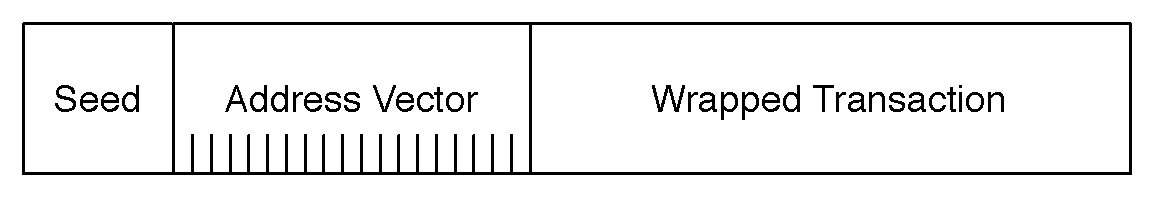
\includegraphics[scale=0.4]{./images/boomerang_message.pdf}
\caption{Boomerang message encoding.}
\label{fig:boomerang_message}
\end{center}
\end{figure}

The procedure to handle Boomerang messages, {\sf BoomerangMessageHandler}, is provided in Algorithm \ref{alg:handler}. 

\begin{algorithm*}[t!]
\caption{{\sf EncodeTransaction}($T$)}
\label{alg:encode}
\begin{algorithmic}[1]

\For{$m = 1$ to $M$}
	\State $\bar{T} := T$
	\State $s \gets \{0,1\}^{\tau}$
	\For{$n = 1$ \textbf{to} $N_m$}
		\State $p := \mathsf{PRG}(s)$
		\State $\bar{T} := \bar{T} \oplus p$
		\State $s \gets E_{pk_{m,n}}(s)$
	\EndFor

	% populate the address vector
	\State $\mathsf{index} \gets \{0,\dots,2N_m\}$ % random address vector index
	\State $\mathsf{AV} := [2N_m]$ % address vector
	\For{$n = N_m$ \textbf{downto} $2$}
		\State $\mathsf{AV}[\mathsf{index}] := E_{pk_{m,n}}(\mathsf{addr}_{N_n})$
		\State $\mathsf{index} := \mathsf{index} + 1 (\mod N_m)$
		\State $\mathsf{AV}[\mathsf{index}] := E_{pk_{m,n}}(\mathsf{addr}_{N_{n-1}})$
		\State $\mathsf{index} := \gets \{0,\dots,2N_m\}$
		\While {$\mathsf{index} \mod 2 \not= 0$ \text{ and } $\mathsf{AV}[\mathsf{index}] \not= \bot \text{ and } \mathsf{AV}[\mathsf{index + 1 (\mod N_m)}] \not= \bot$}
			\State $\mathsf{index} \gets \{0,\dots,2N_m\}$
		\EndWhile
	\EndFor

	\State $M := \mathsf{Pack}(s, \mathsf{AV}, \bar{T})$
	\State $\mathsf{Transmit}(M)$
\EndFor

\end{algorithmic}
\end{algorithm*}

\begin{algorithm*}[t!]
\caption{{\sf BoomerangMessageHandler}($n$, $M$)}
\label{alg:handler}
\begin{algorithmic}[1]

\State $s := D_{sk_{n}}(M[0])$
\State $\bar{T} := M[2] \oplus PRG(s)$
\If {$\bar{T}$ is a well formed transaction}
	\State $\mathsf{Broadcast}(\bar{T})$ to the Bitcoin network
\ElsIf {$\bar{T}$ destination address is $\mathsf{addr}_n$}
	\State Discard $\bar{T}$; return;
\Else
	\State $\mathsf{AV} := M[1]$
	\State $n := 1$
	\While {$n < 2N_m$}
		\State $\mathsf{addr}_{src} := D_{pk_n}(AV[n])$
		\If {$\mathsf{addr}_{src} = \mathsf{addr}_n$}
			\State $\mathsf{addr}_{dst} := D_{pk_n}(AV[n + 1])$
			\State $M := \mathsf{Pack}(s, \mathsf{AV}, \bar{T})$
			\If {$|Buffer| \geq B$}
				\State $\mathsf{Transmit}(M)$
			\Else
				\State $B.add(M)$
			\EndIf
		\Else
			\State $n := n + 2$
		\EndIf
	\EndWhile
\EndIf

\end{algorithmic}
\end{algorithm*}

TODO: cover traffic generation, mix delay

\subsection{Cryptographic Primitives}

TODO: PRG, PK-encryption, etc

% \begin{figure}[ht!]
% \begin{center}
% 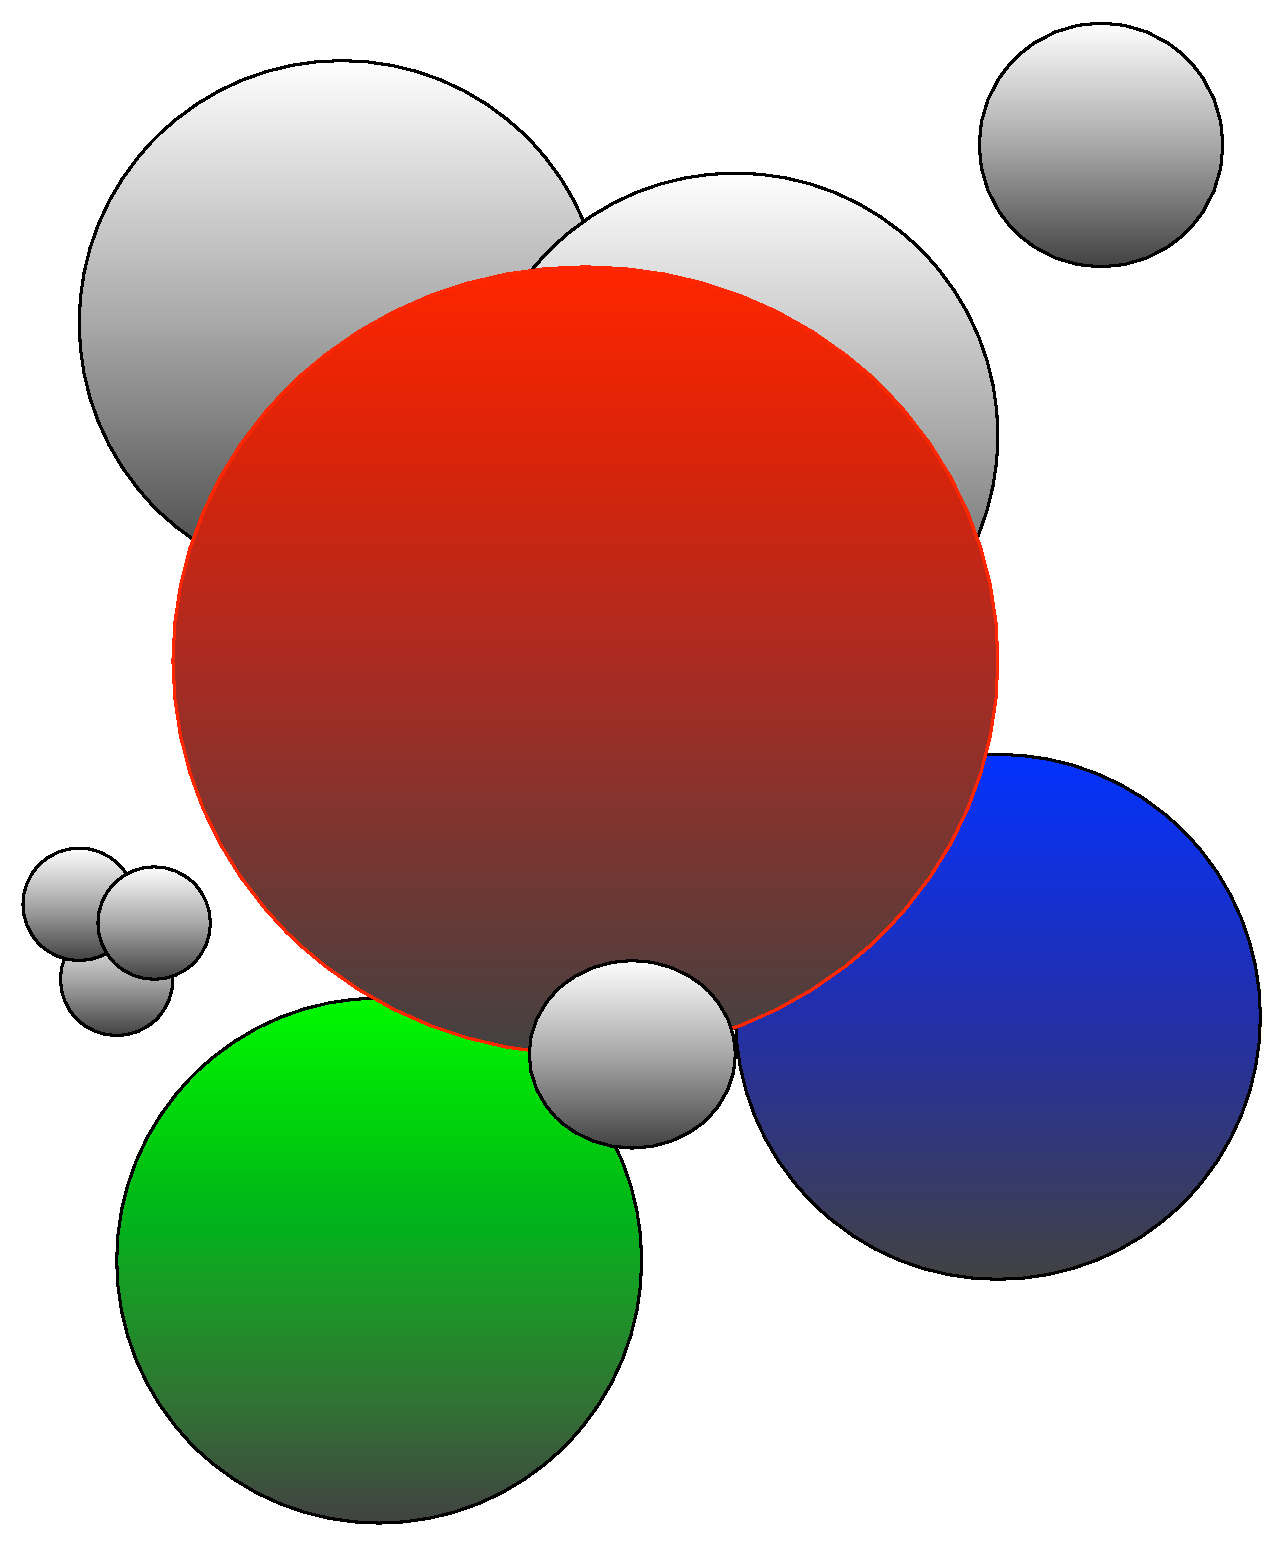
\includegraphics[scale=0.25]{./images/boomerang_clusters.pdf}
% \caption{TODO}
% \label{fig:boomerang_clusters}
% \end{center}
% \end{figure}

\subsection{Parameter Selection}

TODO: discuss parameter selection from below

% cover traffic generation rate (random variable)
% mix buffer delay (random variable)
% circuit length (fixed)
% mix buffer size (fixed)
% encoded transaction size


\section{Simulations and Performance Analysis}
In this section we describe the implementation of our simulator and discuss some performance measurements acquired using this tool. We also describe features that should be added to the simulator to support more realistic experiments. We conclude with a discussion of good parameter selection based on our observations using the simulator.

\subsection{Simulation Design}
To assess the expected overhead introduced by Boomerang we implemented a custom discrete-time simulator that emulates the behavior of Bitcoin nodes (software clients) running Boomerang. Time in the simulation is measured in epochs; at every epoch a series of events occurs that advances the state of the system in some (usually) deterministic way. Our simulator supports the following behavior to closely resemble Boomerang:
\begin{enumerate}
	\item Nodes enter and exit the network at random times. 
	\item Nodes make new transactions using configuration-specificed parameters $W$ and $D$ at a random rate $\pi$.
	\item Nodes generate cover traffic at a random rate $\sigma$.
	\item Nodes manage their internal address address books according the protocol described in section \ref{sec:design}.
\end{enumerate}

In addition, the simulation dynamically computes the following performance metrics:
\begin{enumerate}
	\item Average number of ``computations'' done per node (i.e., the number of public-key encryption operations to encode a transaction).
	\item Total and average message latency from the start to end of a circuit for single and every message, respectively.
	\item Node forwarding throughput (messages/s).
	\item Number of completed messages (transactions and cover messages) vs the number of in-progress messages.
	\item Average number of transaction broadcast retries per node.
\end{enumerate}

The parameters for a particular simulation are specified via a YAML configuration file which is parsed using the Java-based JYaml library \cite{jyaml}. An example configuration file which creates a simulation with $N = 100$ nodes, $D = 6$, $W = 2$, and cover and transaction generation rates uniformly distributed between $[1, 5000]$ and $[1, 7500]$ epochs (i.e., the most granular unit of time).

\begin{lstlisting}
simTime: 2500
numNodes: 100
enterRate: 750
exitRate: 750
gridHeight: 10000
gridWidth: 10000
chaffGenRate: 5000
txGenRate: 7500
circuitWidth: 2
circuitDepth: 6
retryLimit: 7500
buffSize: 10
mixDelay: 50
pktSize: 1024
initialAddressSize: 250
validNodeTransmitReq: 50
addressBookSize: 1000
seed: 256
outfileprefix: "config-out"
path: "."
genMatrices: false
keepInMemory: false
\end{lstlisting}

The {\tt genMatrices} and {\tt keepInMemory} flags are used to ensure that the Java heap space isn't exhausted from memory leaks by storing all of the events generated by the simulation at each time epoch. To run the simulation with 8GB of heap space on the example configuration listed above, which is stored in a local file {\tt config.yaml}, one would run the following command:

\begin{center}
{\small \tt java -cp ./jyaml-1.3.jar:. -Xmx8g Boomerang config.yaml}
\end{center}

\subsection{Performance Metrics and System Parameters}
Using our simulation, we performed a series of small and large experiments; the properties and simulation results for a subset of such experiments are summarized in Tables \ref{tab:experiments} and \ref{tab:sim-results}, respectively. Due to physical memory limitations and the initial single-threaded nature design of our simulator, we could not conduct experiments beyond $N \approx 25000$. We will address this shortcoming in our simulation design for future work. An illustration of cover and transaction messages flowing through the network during the entire duration of Experiment \#1 is shown in Figure \ref{fig:flow}, and a series of smaller windows during which this information is captured is shown in Figure \ref{fig:small-flow}. As expected, the flow of messages appears to be uniformly distributed across all nodes, even when analyzed in small time windows. 

Based on the experimental results and the Boomerang design it is clear that the performance of the Boomerang scheme is tightly coupled to $W$, $D$, and the rate at which cover traffic and new encoded transactions generation ($\sigma$ and $\pi$, respectively). Furthermore, given our anonymity analysis and these performance results, it is clear that we wish to maximize $D$ (circuit depth) and minimize $W$ (circuit width - or the number of independent circuits) so as to reduce the overall work performed by a node while also improving anonymity. However, observe that with few independent circuits of larger depth, the likelihood that a transaction needs to be re-transmitted is increased. This result appeals to intuition since a larger number of hops will ultimately reduce the overall message latency.

To summarize, we recommend that $D$ is maximized, $W$ is minimized, and $\sigma$ is maximized subject to node computational limitations and the expected congestion of the network. Choosing an appropriate value for $\sigma$ should be tied to the expected transaction generation rate $\pi$, which is ultimately controlled by the users, i.e., it is not a system parameter. Unfortunately, we do not have the means to estimate this rate, and thus we leave the selection of the system parameters as future work dependent on such an analysis. 

\begin{table*}
\begin{center}
\caption{Subset of experimental parameters explored with the Boomerang simulator.}
\label{tab:experiments}
    \begin{tabular}{|c|c|c|c|c|c|} \hline
    {\bf Experiment \#} & $N$ & $D$ & $W$ & $\sigma_{max}$ & $\pi_{max}$ \\ \hline
    1 & 50     & 6 & 2 & 5000 & 7500 \\ 
    2 & 100    & 6 & 2 & 5000 & 7500 \\ 
    3 & 150    & 6 & 2 & 5000 & 7500 \\ 
    4 & 200    & 6 & 2 & 5000 & 7500 \\ 
    5 & 250    & 6 & 2 & 5000 & 7500 \\ 
    6 & 1000   & 6 & 2 & 5000 & 7500 \\ 
    7 & 10000  & 6 & 2 & 5000 & 7500 \\ 
    8 & 50     & 8 & 1 & 5000 & 15000 \\ 
    9 & 100    & 8 & 1 & 5000 & 15000 \\ 
    10 & 150   & 8 & 1 & 5000 & 15000 \\ 
    11 & 200   & 8 & 1 & 5000 & 15000 \\ 
    12 & 250   & 8 & 1 & 5000 & 15000 \\ 
    13 & 1000  & 8 & 1 & 5000 & 15000 \\ 
    14 & 10000 & 8 & 1 & 5000 & 15000 \\ 
    \hline
    \end{tabular}
\end{center}
\end{table*}

\begin{table*}
\begin{center}
\caption{Simulation results gathered from the experiment configurations listed in Table \ref{tab:experiments}. Since message latency is not a goal of Boomerang (i.e., the timeliness of transaction broadcasts is not of critical importance), this measurement is omitted for brevity. All simulations were run for a }
\label{tab:sim-results}
% chaff, transaction, num forwarded, number of retries
    \begin{tabular}{|c|c|c|c|c|} \hline
    {\bf Experiment \#} & {\bf Avg. Chaff Generated} & {\bf Avg. Transactions Encoded} & {\bf Avg. Forwarded Messages} & {\bf Avg. Retries} \\ \hline
    1  & ~ & ~ & ~ & ~ \\
    2  & ~ & ~ & ~ & ~ \\
    3  & ~ & ~ & ~ & ~ \\
    4  & ~ & ~ & ~ & ~ \\
    5  & ~ & ~ & ~ & ~ \\
    6  & ~ & ~ & ~ & ~ \\
    7  & ~ & ~ & ~ & ~ \\
    8  & ~ & ~ & ~ & ~ \\
    9  & ~ & ~ & ~ & ~ \\
    10 & ~ & ~ & ~ & ~ \\
    11 & ~ & ~ & ~ & ~ \\
    12 & ~ & ~ & ~ & ~ \\
    13 & ~ & ~ & ~ & ~ \\
    14 & ~ & ~ & ~ & ~ \\


    % 1 & 17.95 & 8.92 & 6008.27 & 0.05 \\ 
    % 2 & 24.12 & 11.36 & 6236.65 & 0.11 \\ 
    % 3 & 29.03 & 14.33 & 9713.91 & 0.06 \\ 
    % 4 & 31.63 & 14.77 & 11466.87 & 0.09 \\ 
    % 5 & 35.32 & 18.70 & 15970.75 & 0.043 \\ 
    % 6 & 35.25 & 18.91 & 16468.7 & 0.04 \\
    % 7 & 29.59 & 20.75 & 13750.8 & 0.02 \\ 
    % 8 & 8.63 & 4.27 & 1262.12 & 0.10 \\ 
    % 9 & 11.93 & 4.35 & 1098.63 & 0.09 \\ 
    % 10 & 12.45 & 5.5 & 1025.23 & 0.14 \\ 
    % 11 & 12.34 & 5.40 & 1442.89 & 0.15 \\ 
    % 12 & 13.70 & 4.92 & 1198.61 & 0.07 \\ 
    % 13 & 15.39 & 6.38 & 1203.95 & 0.17 \\ 
    % \cellcolor{green!25}14 & \cellcolor{green!25}16.21 & \cellcolor{green!25}6.49 & \cellcolor{green!25}1106.63 & \cellcolor{green!25}0.09 \\ 
    \hline
    \end{tabular}
\end{center}
\end{table*}

\begin{figure*}[ht!]
\begin{center}
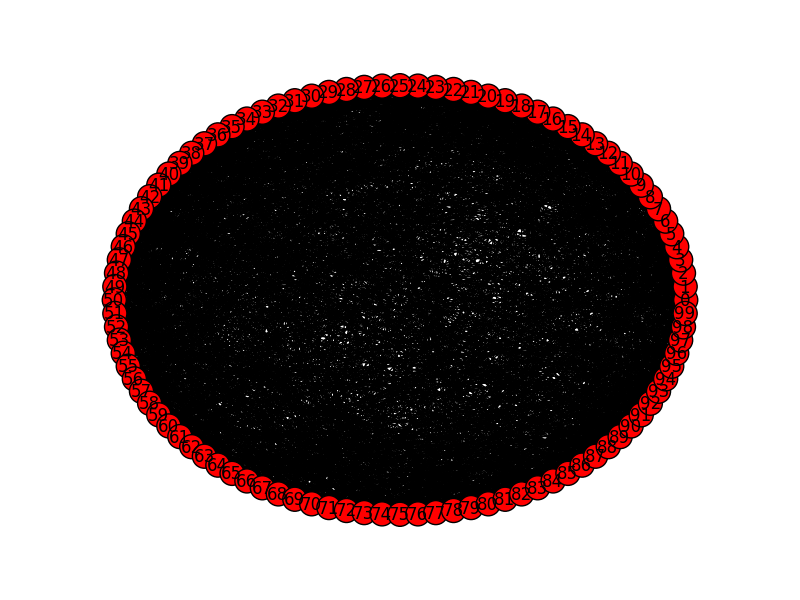
\includegraphics[scale=0.5]{./images/sim1_completedMessage_complete.png}
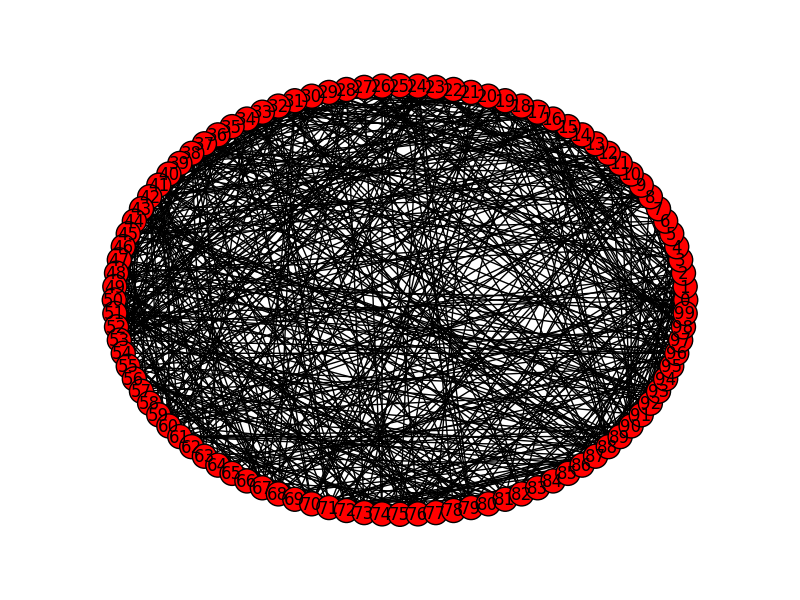
\includegraphics[scale=0.5]{./images/sim1_completedMessage_tx.png}
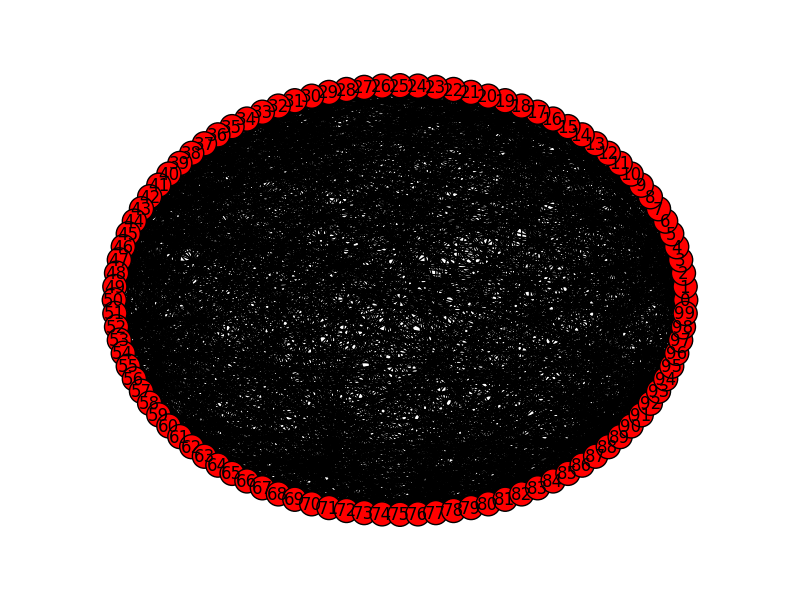
\includegraphics[scale=0.5]{./images/sim1_completedMessage_chaff.png}
\caption{The top figure shows the flow of both dummy messages and forwarded transactions from Experiment \#1, the middle figure shows only the transaction messages, and the bottom figure shows the cover traffic. Nodes have directed edges between them if some message was sent between them during the lifetime of the simulation. The coverage of nodes is clearly uniformly distributed, as desired.}
\label{fig:flow}
\end{center}
\end{figure*}


% cover traffic generation rate (random variable)
% mix buffer delay (random variable)
% circuit length (fixed)
% mix buffer size (fixed)
% encoded transaction size



\begin{thebibliography}{1}

\bibitem{bitcoin} Satoshi Nakamoto. Bitcoin: A Peer-to-Peer Electronic Cash System. \emph{Consulted} 1 (2008).

\bibitem{Chaum81-Mix} David L. Chaum. Untraceable electronic mail, return addresses, and digital pseudonyms. \emph{Communications of the ACM} 24(2) (1981), 84-90.

\bibitem{tarzan} Michael J. Freedman and Robert Morris. Tarzan: A Peer-to-Peer Anonymizing Network Layer. In \emph{Proceedings of the 9th ACM conference on Computer and Communications Security}, ACM (2002).

% \bibitem{chaumain} David L. Chaum. Blind Signatures for Untraceable Payments. \emph{Crypto} 82 (1982).

% \bibitem{zerocoin} Ian Miers, Christina Garman, Matthew Green, Aviel D. Rubin. Zerocoin: Anonymous Distributed E-Cash from Bitcoin. \emph{IEEE Symposium on Security and Privacy} (2013).

% \bibitem{Androulaki12-privacy} Elli Androulaki, Ghassan O. Karame, Marc Roeschlin, Tobias Scherer, and Srdjan Capkun. Evaluating User Privacy in Bitcoin. \emph{IACR Cryptology ePrint Archive} 596 (2012).

% \bibitem{Shamir13-bitcoingraph} Dorit Ron and Adi Shamir. Quantitative Analysis of the Full Bitcoin Transaction Graph. \emph{IACR Cryptology ePrint Archive} 584 (2012).

% \bibitem{ReidHarrigan13} Fergal Reid and Martin Harrigan. An Analysis of Anonymity in the Bitcoin System. \emph{Security and Privacy in Social Networks}, Springer New York (2013), 197-223.

% \bibitem{BetterToBitter} Simon Barber, Xavier Boyen, Elaine Shi, and Ersin Uzun. Bitter to Better -- How to Make Bitcoin a Better Currency. \emph{Financial Cryptography and Data Security}, Springer Berlin Heidelberg (2012), 399-414.

% \bibitem{Fistful12} Sarah Meiklejohn, Marjori Pomarole, Grant Jordan, Kirill Levchenko, Damon McCoyy, Geoffrey M. Voelker, and  Stefan Savage. A Fistful of Bitcoins: Characterizing Payments Among Men with No Names. In \emph{Proceedings of the 2013 Conference on Internet Measurement Conference}, ACM (2013).

% \bibitem{kaminsky} Dan Kaminsky. Black Ops of TCP/IP Presentation. \emph{Black Hat, Chaos Communication
% Camp} (2011).

% \bibitem{bitcoin-tor-wiki} Tor. Bitcoin Wiki. Available online at \url{https://en.bitcoin.it/wiki/Tor}. Last accessed: 1/25/14.

% \bibitem{coinjoin} G. Maxwell. Coinjoin: Bitcoin Privacy for the Real World. Available online at \url{https://bitcointalk.
% org/index.php?topic=279249.0}. Last accessed: 1/31/14.

% \bibitem{pinocchio} George Danezis, C\'{e}dric Fournet, Markulf Kohlweiss, Bryan Parno. Pinocchio Coin: Building Zerocoin from a Succinct Pairing-Based Proof System. In \emph{Proceedings of the First ACM Workshop on Language Support for Privacy-Enhancing Technologies}, ACM (2013).

% \bibitem{mixcoin} Joseph Bonneau, Arvind Narayan, Andrew Miller, Jeremy Clark, and Joshua A. Kroll. Mixcoin - Anonymity for Bitcoin with accountable mixes. Preprint available online at: \url{http://cs.umd.edu/~amiller/mix.pdf}.

% \bibitem{nist-beacon} NIST Randomness Beacon. Available online at: \url{http://www.nist.gov/itl/csd/ct/nist_beacon.cfm}. Last accessed: 2/5/14.

\end{thebibliography}




% that's all folks
\end{document}


